\documentclass[border=6pt,tikz]{standalone}
\usepackage{tikz}
\usepackage{amsmath,amssymb}
\usetikzlibrary{arrows.meta,positioning,fit,backgrounds,calc,shapes.geometric,decorations.pathreplacing,patterns}
\definecolor{ink}{HTML}{1B2430}
\definecolor{muted}{HTML}{6B7785}
\definecolor{accent}{HTML}{2F6FB5}
\definecolor{accent2}{HTML}{C1611F}
\definecolor{good}{HTML}{2E7D5B}
\definecolor{soft}{HTML}{EDF2F7}
\definecolor{soft2}{HTML}{FBEDE2}
\definecolor{soft3}{HTML}{E6F0E9}
\tikzset{
  box/.style={draw=ink,line width=.7pt,rounded corners=2pt,fill=soft,inner sep=4pt,align=center,font=\sffamily\small},
  boxa/.style={box,fill=soft2},
  boxb/.style={box,fill=soft3},
  plain/.style={align=center,font=\sffamily\small,text=ink},
  tiny/.style={align=center,font=\sffamily\scriptsize,text=muted},
  ar/.style={-{Stealth[length=2.4mm]},draw=ink,line width=.7pt},
  arm/.style={-{Stealth[length=2.4mm]},draw=muted,line width=.6pt,dashed},
  nd/.style={circle,draw=ink,line width=.7pt,fill=white,minimum size=7mm,inner sep=0pt,font=\sffamily\scriptsize},
  ndf/.style={nd,fill=soft},
  ndt/.style={nd,fill=soft2},
}

\begin{document}
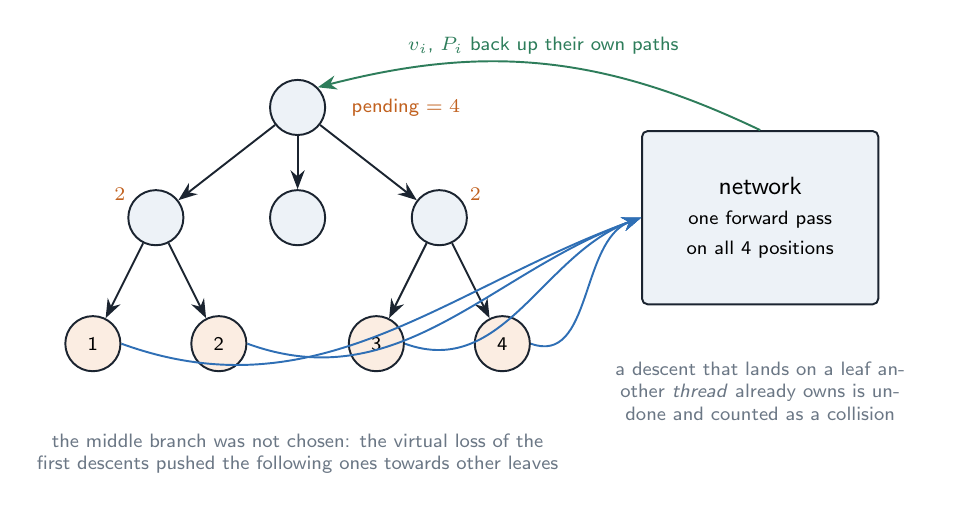
\begin{tikzpicture}[x=1mm,y=1mm]
  \node[ndf] (r) at (30,40) {};
  \node[ndf] (a) at (12,26) {}; \node[ndf] (b) at (30,26) {}; \node[ndf] (c) at (48,26) {};
  \node[ndt] (l1) at (4,10) {1}; \node[ndt] (l2) at (20,10) {2}; \node[ndt] (l3) at (40,10) {3}; \node[ndt] (l4) at (56,10) {4};
  \draw[ar] (r)--(a); \draw[ar] (r)--(b); \draw[ar] (r)--(c);
  \draw[ar] (a)--(l1); \draw[ar] (a)--(l2); \draw[ar] (c)--(l3); \draw[ar] (c)--(l4);
  \node[tiny,right=1mm of r,text=accent2,xshift=1mm] {pending $=4$};
  \node[tiny,left=0mm of a,text=accent2,xshift=1mm,yshift=3mm] {$2$};
  \node[tiny,right=0mm of c,text=accent2,xshift=-1mm,yshift=3mm] {$2$};
  \node[tiny] at (30,-4) {the middle branch was not chosen: the virtual loss of the\\first descents pushed the following ones towards other leaves};

  \node[box,right=22mm of c,minimum width=30mm,minimum height=22mm,anchor=west] (nn)
    {network\\\scriptsize one forward pass\\\scriptsize on all 4 positions};
  \foreach \l in {l1,l2,l3,l4} \draw[ar,draw=accent] (\l.east) to[out=-20,in=200] (nn.west);
  \draw[ar,draw=good] (nn.north) to[bend right=20] node[tiny,above,text=good]{$v_i$, $P_i$ back up their own paths} (r.north east);
  \node[tiny,below=6mm of nn,text width=44mm] {a descent that lands on a leaf another
    \emph{thread} already owns is undone and counted as a collision};
\end{tikzpicture}
\end{document}
